\chapter{El disco de Poincaré}
\label{cap:disco-poincare}

El disco de Poincaré representa el plano hiperbólico mediante el disco unitario abierto
\[
  \mathbb{D}=\{z\in\mathbb{C}:|z|<1\}.
\]
La frontera circular no forma parte del plano; sus puntos se interpretan como puntos ideales. Aunque el dibujo cabe en una región finita, la distancia hiperbólica hacia la frontera es infinita \cite{anderson2005}.

\section{La métrica}

La métrica de Poincaré asigna a un desplazamiento infinitesimal la longitud
\begin{equation}
  ds^2=\frac{4\,|dz|^2}{(1-|z|^2)^2}.
  \label{eq:metrica-poincare}
\end{equation}
El factor del denominador crece al acercarse a \(|z|=1\). Por eso, segmentos euclidianos de tamaño parecido pueden tener longitudes hiperbólicas muy distintas según dónde estén situados.

La distancia entre dos puntos \(z,w\in\mathbb{D}\) satisface
\begin{equation}
  \cosh d_{\mathbb{D}}(z,w)
  =1+\frac{2|z-w|^2}{(1-|z|^2)(1-|w|^2)}.
  \label{eq:distancia-poincare}
\end{equation}
En particular, desde el origen se obtiene \(d_{\mathbb{D}}(0,z)=2\operatorname{artanh}|z|\), que diverge cuando \(|z|\) tiende a uno.

\section{Geodésicas}

Las geodésicas del disco son los diámetros y los arcos de circunferencias que cortan la circunferencia unidad en ángulo recto. En la \cref{fig:disco-poincare} el diámetro es una geodésica y el arco rojo pertenece a una circunferencia ortogonal a la frontera.

\begin{figure}[htbp]
  \centering
  % Fragmento reutilizable: se incorpora desde un entorno figure con \input.
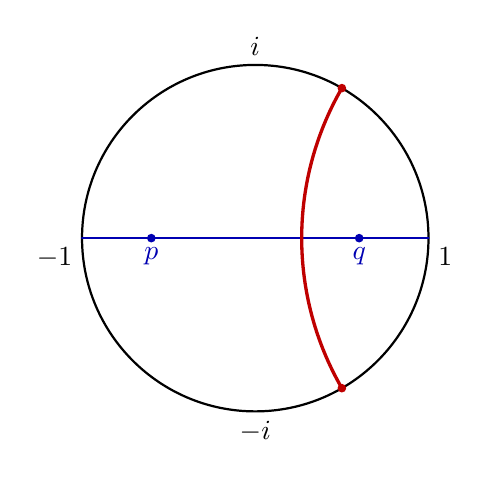
\begin{tikzpicture}[scale=2.2,line cap=round]
  \draw[thick] (0,0) circle (1cm);
  \draw[blue!70!black,thick] (-1,0) -- (1,0);
  % Arco de la circunferencia de centro (2,0) y radio sqrt(3): ortogonal al borde.
  \draw[red!75!black,very thick]
    (0.5,0.8660254) arc[start angle=150,end angle=210,radius=1.7320508cm];
  \fill[blue!70!black] (-0.6,0) circle (0.025) node[below] {$p$};
  \fill[blue!70!black] (0.6,0) circle (0.025) node[below] {$q$};
  \fill[red!75!black] (0.5,0.8660254) circle (0.025);
  \fill[red!75!black] (0.5,-0.8660254) circle (0.025);
  \node[below left] at (-1,0) {$-1$};
  \node[below right] at (1,0) {$1$};
  \node[above] at (0,1) {$i$};
  \node[below] at (0,-1) {$-i$};
\end{tikzpicture}

  \caption{Geodésicas en el disco de Poincaré.}
  \label{fig:disco-poincare}
\end{figure}

La geometría del modelo conserva los ángulos: el ángulo entre dos curvas medido en el disco coincide con el ángulo hiperbólico entre ellas. Las longitudes, en cambio, se miden con la métrica \cref{eq:metrica-poincare}, no con la distancia euclidiana del dibujo.

\section{Transformaciones que conservan la métrica}

Las transformaciones de Möbius
\[
  T_a(z)=e^{i\theta}\frac{z-a}{1-\overline{a}z},
  \qquad |a|<1,
\]
envían el disco en sí mismo y preservan la métrica hiperbólica. En particular, permiten trasladar cualquier punto del disco al origen sin cambiar distancias ni ángulos \cite{anderson2005,stillwell2005}.

\begin{example}[Distancia radial]
Para \(r\in[0,1)\), la distancia del origen al punto real \(r\) es \(2\operatorname{artanh}(r)\). Al crecer \(r\), la distancia crece sin cota aunque el punto permanezca dentro del círculo euclidiano.
\end{example}
